\documentclass[kulak]{kulakarticle} % options: kulak (default) or kul

\usepackage[dutch]{babel}
\usepackage{graphicx}
\usepackage{amssymb, amsthm, amsmath}
\usepackage{url}

\title{Hoe kan de veiligheid van fietsers verbeterd worden met slimme sensoren?}
\author{Vincent Van Schependom}
\date{Academiejaar 2023 -- 2024}
\address{
	\textbf{Groep Wetenschap \& Technologie Kulak}\\
	Informatica\\
	Wetenschappelijk Schrijven }
	

\begin{document}

\maketitle

\section*{Inleiding}

De laatste jaren heeft de fietsindustrie een enorme vlucht genomen. In tijden van klimaatopwarming en economische crisis, kiezen mensen wereldwijd voor een duurzamere, actievere en meer economische manier om zich te verplaatsen. Maar is de fiets ook een veiliger transportmiddel dan pakweg een auto? Helaas zijn verkeersongevallen met fietsers niet weg te denken uit de media. Bovendien bereiken ons maar al te vaak droevige overlijdensberichten van wielrenners die zijn omgekomen in het verkeer. De kwestie rond veiligheid van fietsers is dus urgent. Hoe kunnen we, door middel van sensoren, zorgen voor een betere  preventie van verkeersongevallen met fietsers? Hoe kunnen we bovendien zo'n ongeval detecteren indien het zich toch zou voordoen?

\section{Preventie van ongevallen}

\subsection{Werking van het preventiemechanisme}

Radartechnologie is absoluut geen baanbrekende nieuwigheid, het wordt namelijk al langer gebruikt in onder andere de auto-industrie. De technologie kan, door middel van golven, objecten detecteren en bijkomende informatie te weten komen over deze objecten, zoals afstand tot de sensor, snelheid, etc. In de fietsindustrie worden zo'n sensoren nu volop ontwikkeld in kleinere formaten. Op die manier kunnen ze geïntegreerd worden in apparaten die standaard al gebruikt worden door fietsers, zoals bijvoorbeeld achterlichten.

Radarsensoren steunen op het verschil in de frequentie van het uitgezonden golfsignaal en die van het ontvangen golfsignaal. Beide frequenties verschillen van elkaar ten gevolge van het dopplereffect. We kunnen dit effect specifiek toepassen op de situatie van een auto die tot een fietser nadert langs achter, om op die manier de snelheid van de auto te bepalen. Een illustratie hiervan is te zien in figuur \ref{fig:doppler}.

\subsection{Het dopplereffect toegepast}

In situatie 1 zendt de radar in het achterlicht van de fietser golven uit met frequentie \(f_{r1}\). De auto is in dit geval de (bewegende) waarnemer en de radar is de (bewegende) bron. Door het dopplereffect is de frequentie \(f_a\) die de auto zal waarnemen groter dan de frequentie \(f_{r1}\) die wordt uitgezonden door de radar.

In situatie 2 weerkaatst de auto de opgevangen golven van situatie 1. De auto is nu dus de (bewegende) bron en de radar is nu de (bewegende) ontvanger. Er is in deze situatie ook sprake van het dopplereffect, waardoor de waargenomen frequentie \(f_{r2}\) zal verschillen van de uitgezonden frequentie \(f_a\).

Steunend op de formules uit het practicum over het dopplereffect van \textit{Conceptuele Natuurkunde}  \cite{practicumdoppler}, waarbij zowel de bron als de waarnemer bewegen, kunnen we nu de snelheid van de auto bepalen. Door de waargenomen frequentie \( f_a=f_{r1}\cdot \left( \frac{c+v_a}{c-v_f} \right) \) van de eerste situatie en de waargenomen frequentie \( f_{r2}=f_a\cdot \left( \frac{c+v_f}{c-v_a} \right) \) van de tweede situatie te combineren, kan de radar de snelheid van de auto \[v_a = c \cdot \left( \frac{f_{r2}-f_{r1}}{f_{r2}+f_{r1}} \right)\cdot \left(\frac{c-v_f}{c+v_f} \right)\] bepalen. Hierbij zijn \(v_f\) de snelheid van de fietser en \(c\) de voortplantingssnelheid van de golven door het medium, in dit geval lucht.

\newpage

\begin{figure}
	\centering
	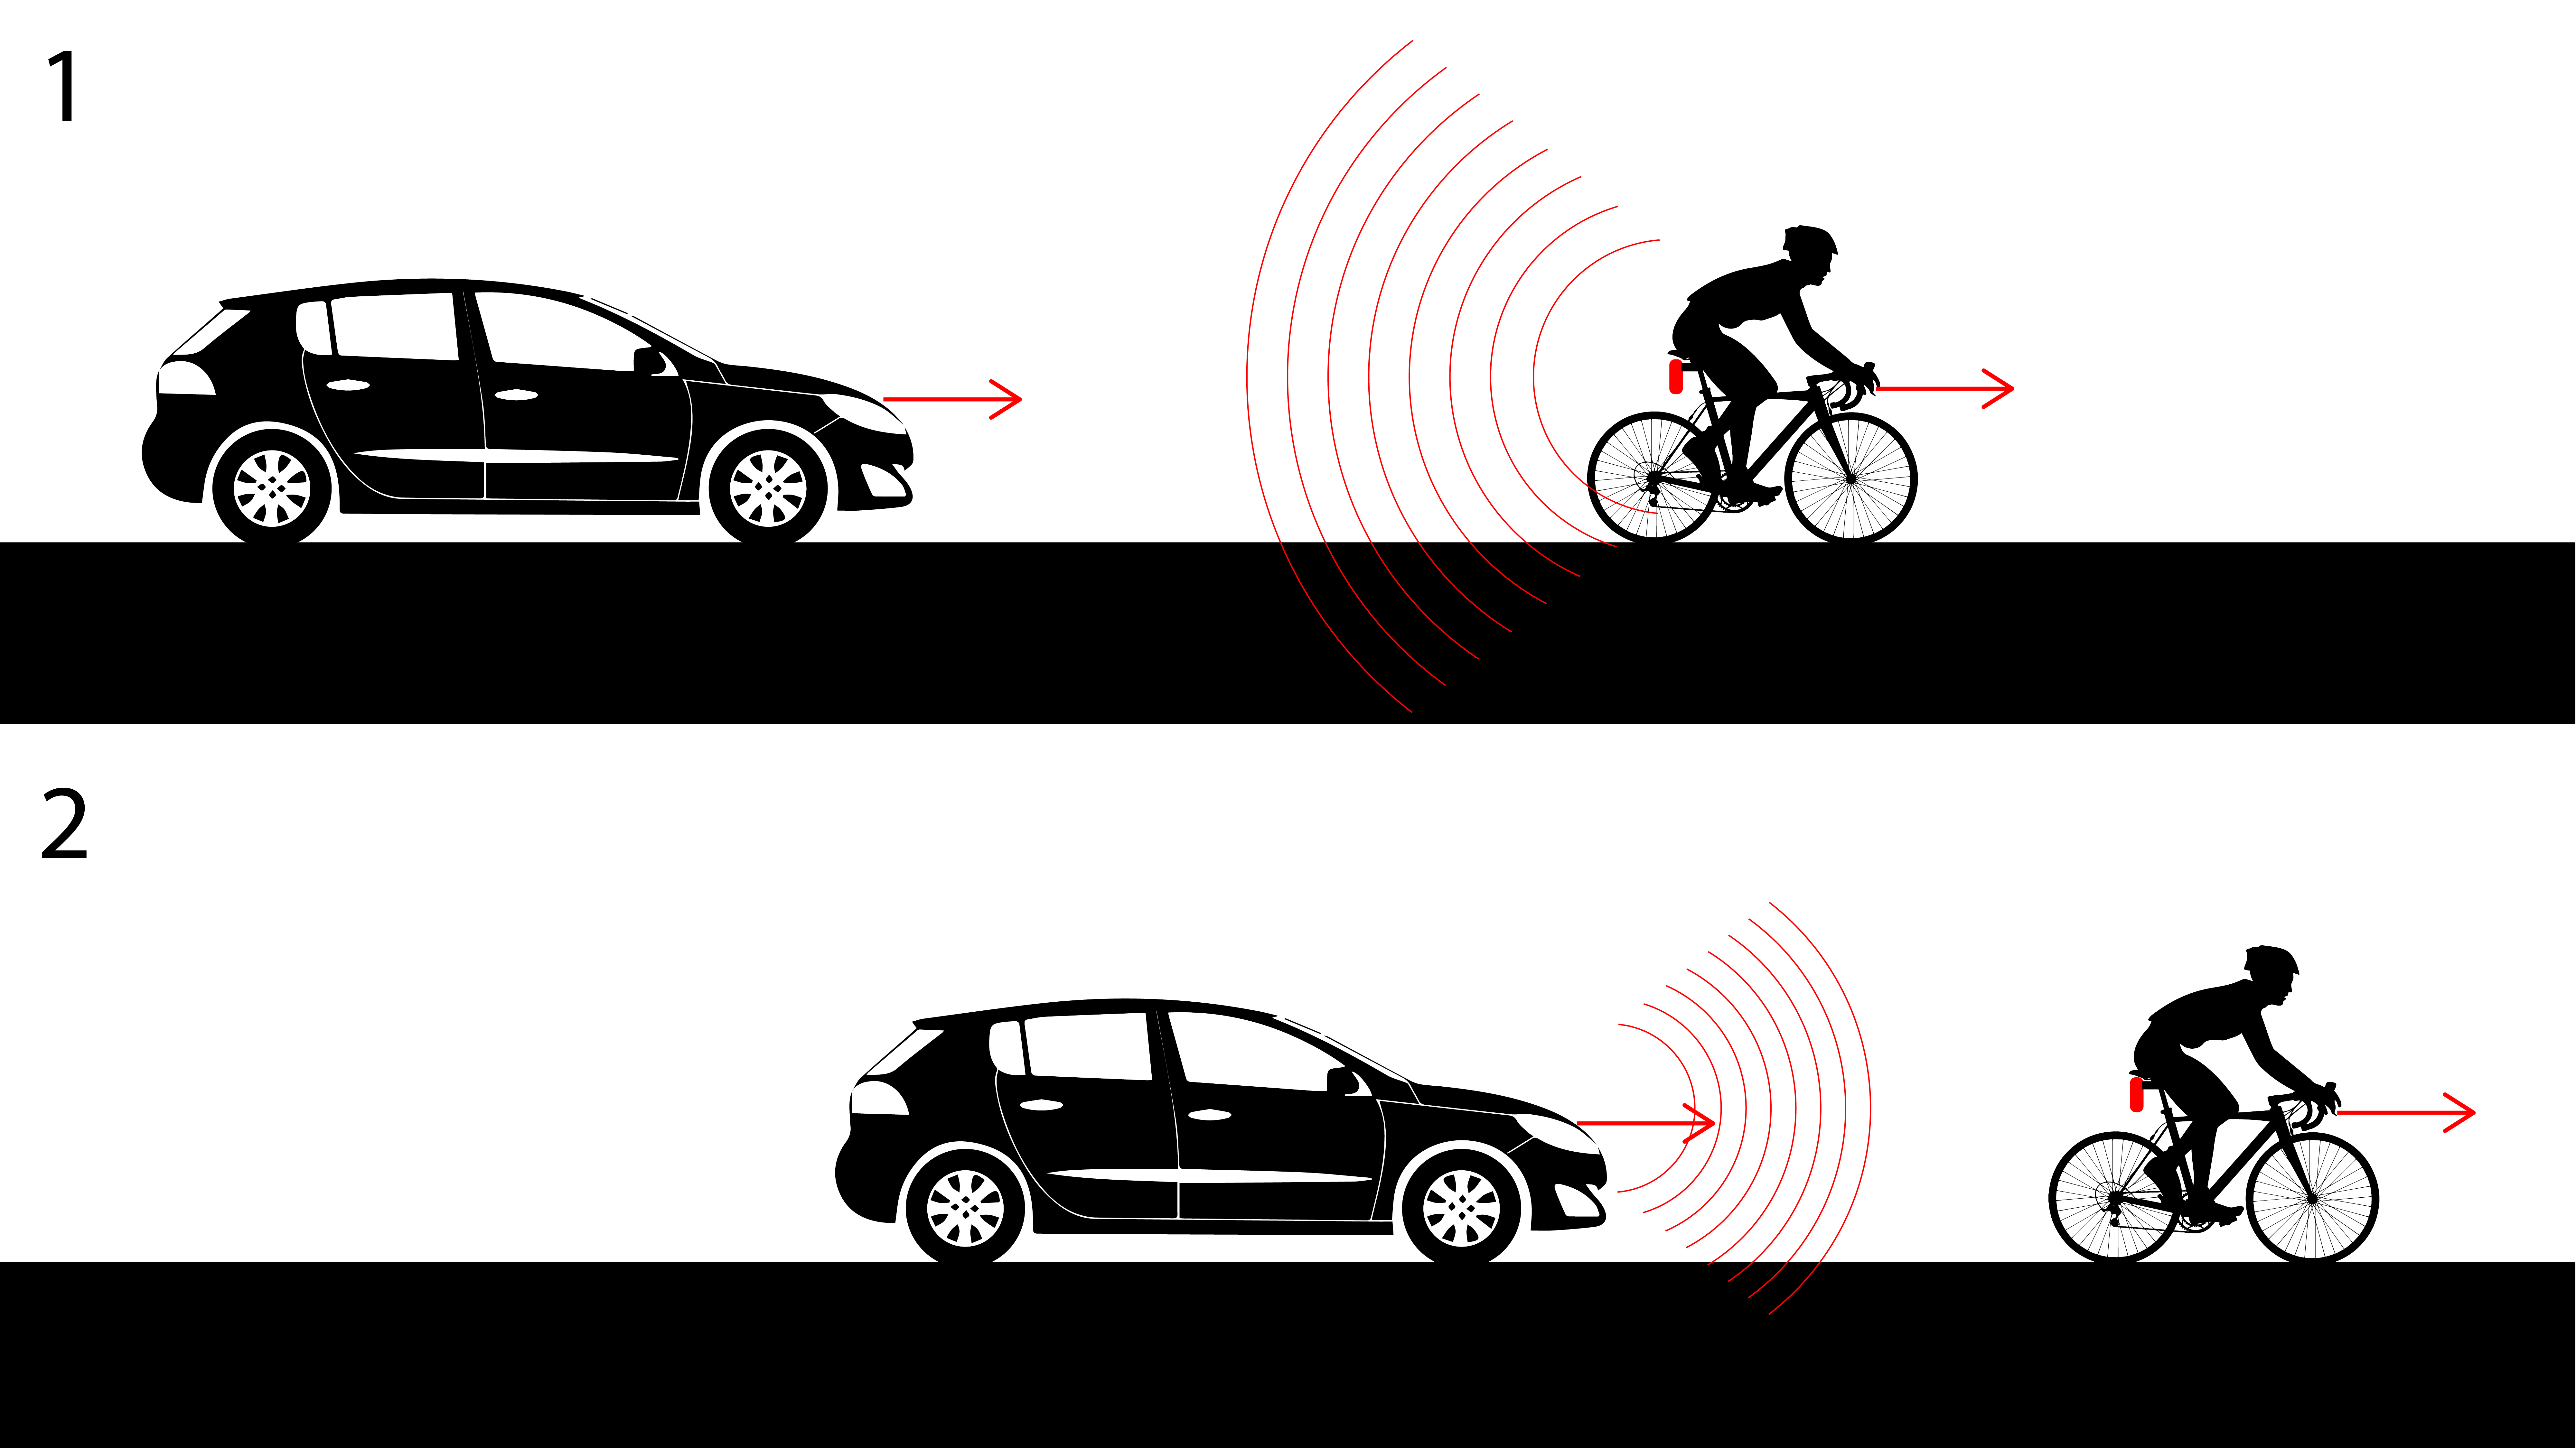
\includegraphics[width=.7\textwidth]{doppler.jpg}
	\caption{Een auto die tot een fietser, met een radar in het achterlicht, nadert. Beide objecten zijn in beweging en er is bij beide situaties sprake van een frequentieverschuiving ten gevolge van het dopplereffect. In situatie 1 is de auto de waarnemer en is de radar de bron. In situatie 2 is de radar de waarnemer en is de auto de bron, die de golven uit situatie 1 weerkaatst.}
	\label{fig:doppler}
\end{figure}

\section{Detectie van ongevallen}

Als er zich toch een ongeval voordoet, is het belangrijk dat de juiste hulp zo snel mogelijk wordt ingeschakeld. Volgens een analyse neemt de kans op het redden van iemands leven met zes procent toe als de responstijd bij noodsituaties met slechts één minuut zou worden verkort \cite{KhanArsalan2018Adas}. Indien de fietser bewusteloos zou zijn en er geen omstaanders zouden zijn, kan die korte responstijd niet gegarandeerd worden en moeten we dus op zoek naar oplossingen.

\subsection{Wetenschappelijk onderzoek}

Er werden vanuit wetenschappelijke hoek reeds verschillende voorstellen gedaan i.v.m. de ontwikkeling van apparaten die fietsongevallen kunnen detecteren, om zo een oplossing te bieden voor dit probleem. Een aantal onderzoekers aan de universiteit van Maleisië stelden bijvoorbeeld een systeem voor dat gebruik maakt van een versnellingsmeter om een mogelijke crash te detecteren \cite{KitTamJun2023CFDS}. 

Deze sensoren worden in het onderzoek gekoppeld met het IoT (\textit{Internet of Things}). IoT verwijst naar het netwerk van voorwerpen waarin sensoren, software en andere technologieën zijn verwerkt om via het internet verbinding te maken met elkaar en gegevens uit te wisselen met andere apparaten en systemen. In dit onderzoek wordt dit netwerk gebruikt om, na het detecteren van een ongeval, alarm te slaan en hulp in te schakelen.

\subsection{Reeds verkrijgbare sensoren}

Dergelijke crashsensoren zijn intussen ook commercieel verkrijgbaar. Zo ontwikkelde het Amerikaanse bedrijf Specialized Bicycle Components hun ANGi-sensor, die gelijkaardige technologieën gebruikt en bovendien gekoppeld kan worden aan de smartphone van de gebruiker. In het geval van een crash verwittigt de sensor, die aan de helm van het slachtoffer bevestigt zit, de noodcontacten die opgegeven werden in de bijhorende app.

Deze sensoren schieten vaak nog te kort op vlak van nauwkeurigheid. Zo kan een ongeval gedetecteerd worden wanneer het zich helemaal niet heeft voorgedaan. Dit is op zich geen al te groot probleem, aangezien de gebruiker de noodoproep binnen de 10 seconden kan annuleren. Het omgekeerde kan echter ook optreden, namelijk dat er zich een ongeval voordoet en dat de sensor dit helemaal niet opmerkt, wat natuurlijk veel problematischer is. Er zal dus nog gewerkt moeten worden aan de accuraatheid van deze technologie.

\section*{Besluit}

De ontwikkeling van preventietechnologieën, zoals radars in het achterlicht van fietsers, is ondertussen ver gevorderd. Steunend op het dopplereffect, kunnen dit soort apparaten aan wielrenners en alledaagse fietsgebruikers een extra indicator bieden voor naderend verkeer en zo hun verkeersveiligheid bevorderen.

Ook de ontwikkeling van crashsensoren staat niet stil. Deze technologie is vaak echter niet nauwkeurig genoeg om ten volle op te kunnen vertrouwen. Het blijft helaas moeilijk om zowel het aantal valspositieve metingen als het aantal ongedetecteerde crashes te minimaliseren.

\nocite{TabeiFatemehsadat2021ADSf}

\bibliographystyle{unsrt}
\bibliography{bibliografie}

\end{document}
